%
% user_manual.tex
%
% Copyright (C) 2019 by Gabriel Mariano Marcelino <gabriel.mm8@gmail.com>.
%
% Relatório 3 do Trabalho Final da Disciplina EEL510265.
%
% This work is licensed under the Creative Commons Attribution-ShareAlike 4.0
% International License. To view a copy of this license,
% visit http://creativecommons.org/licenses/by-sa/4.0/.
%

%
% \brief User manual appendix.
%
% \author Gabriel Mariano Marcelino <gabriel.mm8@gmail.com>
%
% \version 0.1.0
%
% \date 21/11/2019
%

\newpage

\section*{Manual do Usuário} \label{sec:user_manual}

Neste apêndice encontra um manual de usuário preliminar do sistema.

\subsection{Compilando o Código Fonte}

Para compilar o código fonte, há dois procedimentos diferentes (um para cada tipo de plataforma alvo). Para a versão a ser executada em um microcomputador, é necessário o compilador ``gcc''\footnote{Procedimento testado utilizando a versão 9.2.1.}. Com o compilador instalado, basta abrir um terminal na pasta onde encontra-se o código fonte e executar o comando ``\textit{make}'', como pode ser visto na \autoref{fig:cmd-make}.

\begin{figure}[!ht]
    \begin{center}
        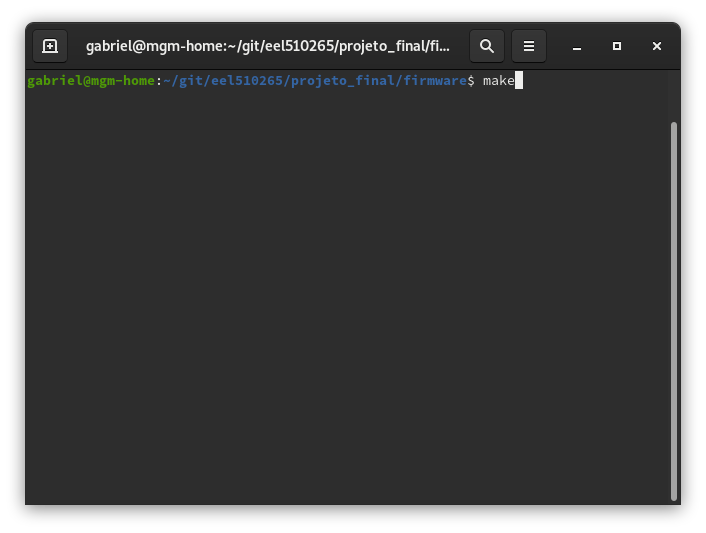
\includegraphics[width=0.75\textwidth]{figures/window_make.png}
        \caption{Terminal com o comando necessário para compilar o código fonte.}
        \label{fig:cmd-make}
    \end{center}
\end{figure}

\subsection{Executando o Código em um Microcomputador}

Após compilar o código fonte, para rodar o programa basta executar o comando ``\textit{./vending-machine}''. Este procedimento encontra-se ilustrado na \autoref{fig:cmd-exec}.

\begin{figure}[!ht]
    \begin{center}
        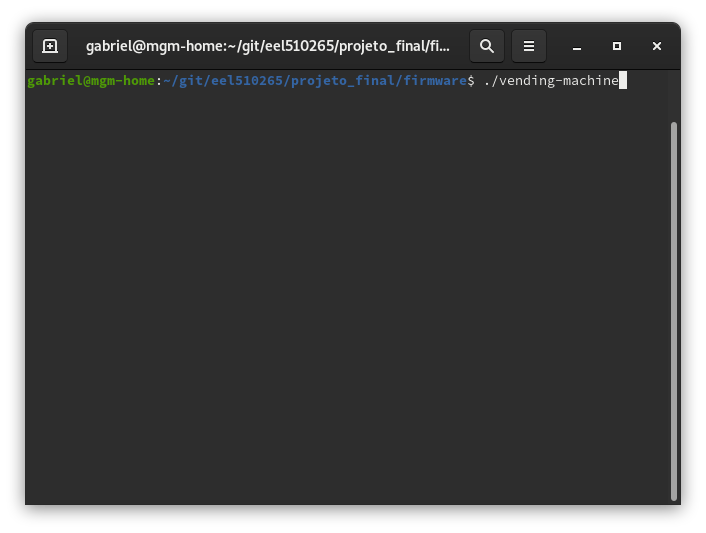
\includegraphics[width=0.75\textwidth]{figures/window-cmd-exec.png}
        \caption{Terminal com o comando necessário para executar o programa após a compilação.}
        \label{fig:cmd-exec}
    \end{center}
\end{figure}
